\section{Parallelismo}
A partire dal 1971 si è sempre rivelata vera la \textit{Legge di Moore} che afferma: "Il numero di transistor per chip, raddoppia ogni 18 mesi".

\spacer
Negli anni i progettisti di processori hanno affrontato con svariate tecniche il problema di tradurre l'aumento di densità dei transistor in un aumento delle prestazioni.

Ogniuna di queste tecniche ha pro e contro:
\spacer
\begin{sitemize}
    \item \textbf{Ridurre il numero di cicli}, quindi migliorare gli algoritmi. Questa è ancora una strada percorribile, ma in 60 anni di ricerca nell'ambito siamo riusciti a trovare soluzioni ottime per i problemi più rilevanti sull'ambito.
    \item \textbf{Aumentare la frequenza di clock} si rivela problematico per l'aumento di calore che viene prodotto, i processori moderni già producono la massima quantità di calore che può essere praticamente dissipata.
    \item Il \textbf{Parallelismo} è la strada che si è intrapresa negli ultimi anni, ha lo svantaggio di richiedere dell'overhead, quindi raddoppiare il numero di core non raddoppia le prestazioni, ma è la strada che permette di sfruttare l'aumento di densità nei transistor.

    Il parallelismo può avvenire al livello dell'istruzione, permettendo più operazioni all'interno dello stesso core (pipeline). Oppure può avvenire a livello di core, inserendo più core.
\end{sitemize}

\spacer
I metodi più utilizzati per realizzare il parallelismo sono:

\spacer
\begin{sitemize}
    \item \textbf{Componenti piccole} che \textbf{interagiscono fortemente tra loro}.

    Con questa soluzione viene parallelizzata la singola operazione (\textit{parallelismo fine-grained})

    Un esempio si trova nell'hyperthreading che permette ad una CPU di eseguire più processi allo stesso tempo.

    \item Un \textbf{piccolo numero di CPU grandi} dotate di \textbf{interconnessioni a bassa velocità}.

    Con questa tecnica l'elemento che viene parallelizzato è l'intero processo  (\textit{parallelismo course-grained})

    Ne sono esempi i sistemi multicore e la realizzazione di chip dedicati a specifiche operazioni.

\end{sitemize}

\begin{figure}[H]
    \centering
    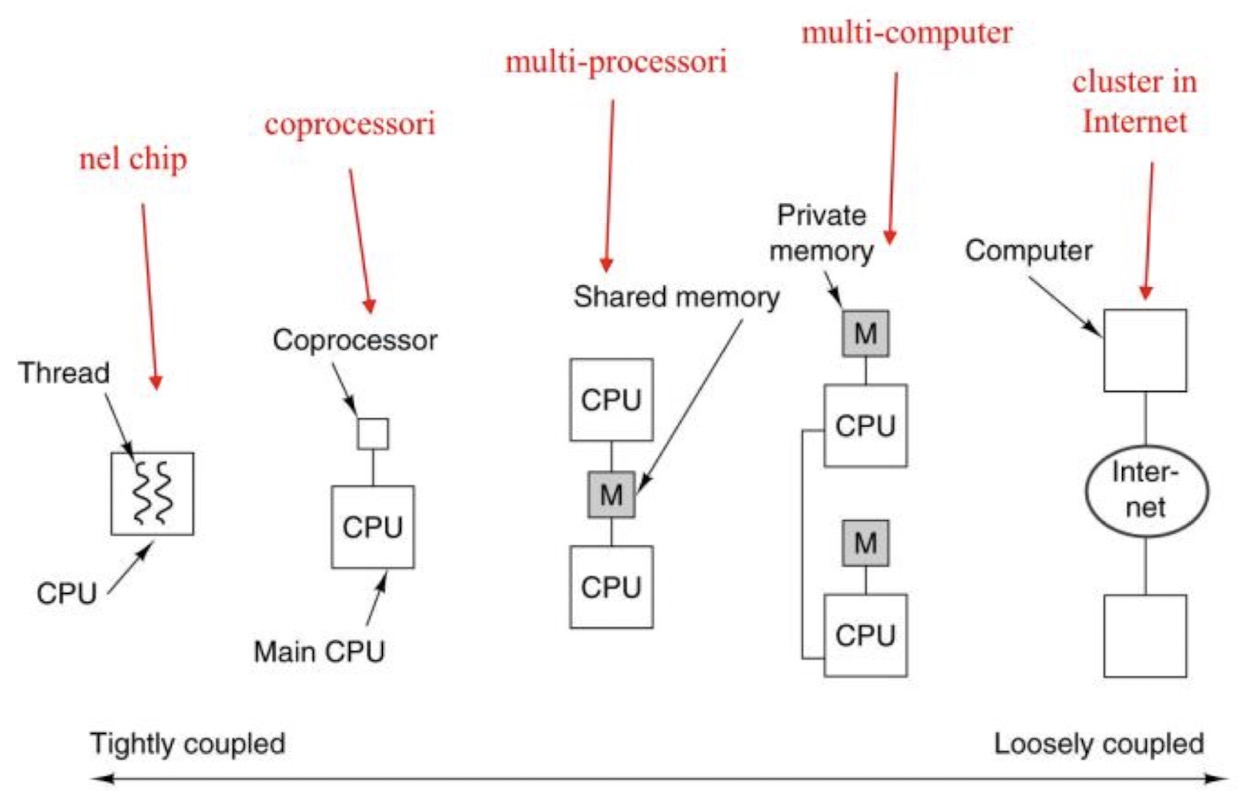
\includegraphics[width=0.45\linewidth]{assets/parallellismo.jpg}
\end{figure}

Gli elementi che caratterizzano il parallelismo, dal punto di vista hardware sono:
\begin{sitemize}
    \item \textbf{Natura e numero degli elementi di calcolo}, pochi elementi a prestazioni elevate, oppure molti elementi a basse prestazioni
    \item \textbf{Natura e numero degli elementi di memoria} La memoria viene divisa in moduli per permetterne l'accesso a tutti gli elementi di calcolo, il modo in cui viene divisa influenza il parallelismo
    \item \textbf{Modalità di connessione} Le connessioni possono essere di tipo statico, oppure dinamico, gestite tramite uno switch in grado di instradare i messaggi.
\end{sitemize}

\subsection{Implementazioni}
Il parallelismo può essere quindi implementato su più livelli:
\begin{sitemize}
    \item \textbf{A livello di istruzioni} tramite pipeline.
    \item \textbf{Multi-threading} Due thread vengono eseguiti contemporaneamente, una CPU virtualizza due CPU.
    \item \textbf{Multi-core} Consente il completo multi-threading di più processi.
    \item \textbf{Core Eterogenei} all'interno dello stesso chip, ogniuno con funzionalità specializzate.
\end{sitemize}

\begin{note}
    Sia intel (a partire dall'architettura Ice Lake) che Apple (con i suoi Apple Silicon), implementano un'architettura ibrida, con core ad alte prestazioni e altri core per processi di minore importanza.
\end{note}